\documentclass{beamer}
\mode<presentation>
\usetheme{CambridgeUS}
\usepackage[russian]{babel}
\usepackage[utf8]{inputenc}
\usepackage[T2A]{fontenc}
\usepackage{sansmathaccent}

\usepackage{verbatim}
\usepackage{alltt}

\pdfmapfile{+sansmathaccent.map}
\title[Межпроцессное взаимодействие]{Сокеты}
\author{Наумов Д.А., доц. каф. КТ}
\date[26.11.2019] {Операционные системы и системное программное обеспечение, 2019}

\begin{document}

%ТИТУЛЬНЫЙ СЛАЙД
\begin{frame}
  \titlepage
\end{frame}
  
%СОДЕРЖАНИЕ ЛЕКЦИИ
\begin{frame}
  \frametitle{Содержание лекции}
  \tableofcontents  
\end{frame}

\section{Сокеты}

\subsection{Удаленное межпроцессное взаимодействие}

\begin{frame}
	Удаленное межпроцессное взаимодействие осуществляется \textit{через сеть} посредством \textit{сокетов}.
	\begin{block}{Сокет}
		комплексное понятие, которое условно можно назвать <<точкой соединения процессов>>.
	\end{block}
	\begin{figure}[h]
		\centering
	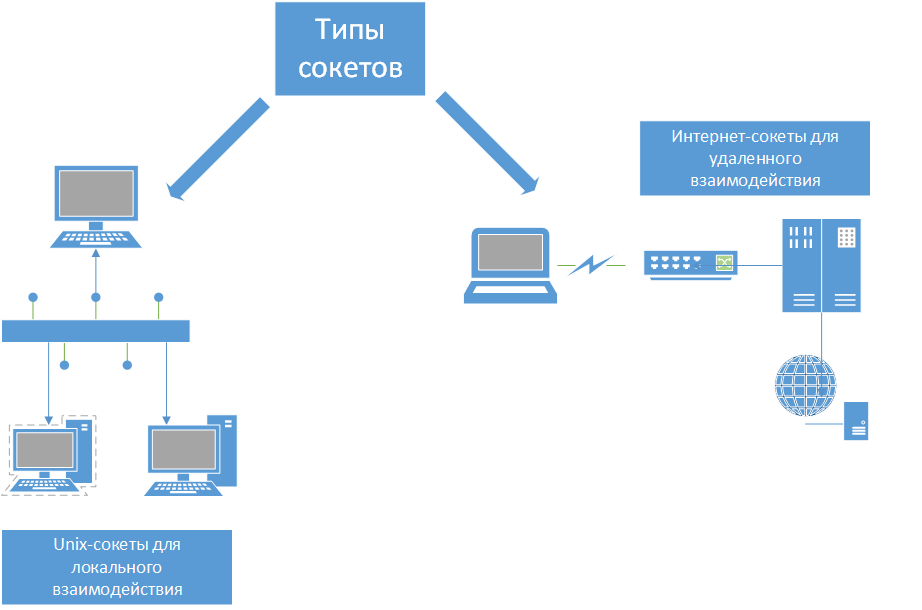
\includegraphics[scale=0.35]{images/lec12-pic01.png}
	\end{figure}
\end{frame}

\begin{frame}
Осбенности использования сокетов:
\begin{itemize}
\item сокеты фигурируют в виде \textit{файловых дескрипторов}, над которыми (во многих случаях) можно осуществлять обычные операции чтения-записи (read(), write() и т. д.);
\item набор действий, подготавливающих файловый дескриптор к использованию, несколько сложнее, чем в случае с обычными файлами;
\item при взаимодействии посредством сокетов процессы рассматриваются по схеме \textit{<<клиент — сервер>>};
\item процесс-сервер устанавливает <<правила общения>> и предлагает всем желающим межпроцессное взаимодействие.
\end{itemize}
\end{frame}

\begin{frame}{Работа с сокетами на стороне сервера}
	\begin{figure}[h]
		\centering
	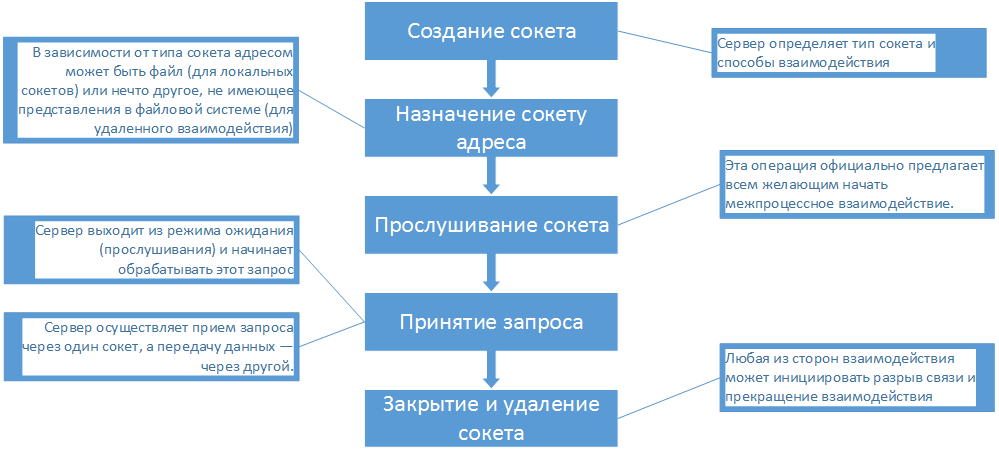
\includegraphics[scale=0.45]{images/lec12-pic02.png}
	\end{figure}
\end{frame}

\begin{frame}{Работа с сокетами на стороне клиента}
	\begin{figure}[h]
		\centering
	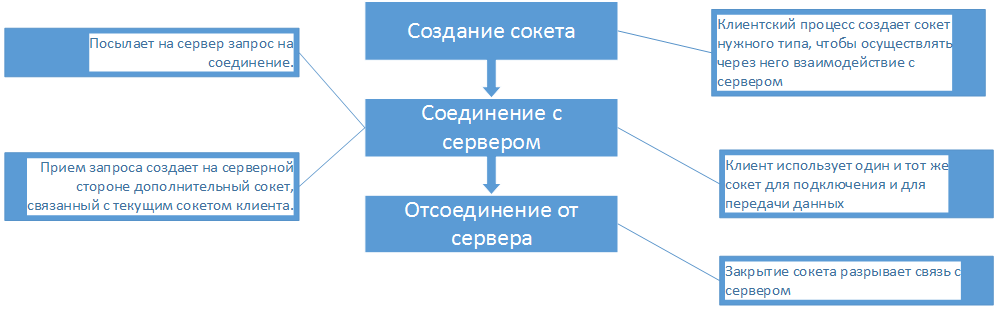
\includegraphics[scale=0.45]{images/lec12-pic03.png}
	\end{figure}
\end{frame}

\subsection{Виды сокетов}

\begin{frame}
	\begin{figure}[h]
		\centering
	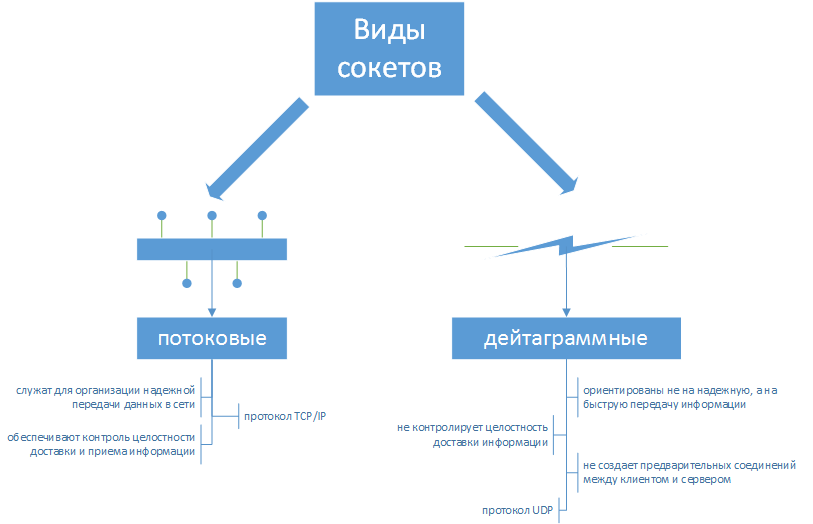
\includegraphics[scale=0.5]{images/lec12-pic04.png}
	\end{figure}
\end{frame}

\subsection{Создание сокетов}

\begin{frame}[fragile]{Создание сокетов}
	Для создания сокетов предназначен системный вызов socket():
	\begin{alltt}
		int socket (int PF, int SOCK\_TYPE, int PROTOCOL)
	\end{alltt}
	\begin{itemize}
		\item при успешном завершении возвращает дескриптор сокета (признак ошибки -1);
		\item PF - семейство протоколов сокета;
		\begin{itemize}
			\item PF\_LOCAL, PF\_UNIX - локальные сокеты (Unix-сокеты);
			\item PF\_FILE - нестандартный синоним PF\_LOCAL;
			\item PF\_INET - интернет-сокеты, основанные на IP версии 4;
			\item PF\_INET6 - интернет-сокеты, основанные на IP версии 6;
			\item PF\_BLUETOOTH - bluetooth-сокеты.
		\end{itemize}
		\item SOCK\_TYPE - способ взаимодействия;
		\begin{itemize}
			\item SOCK\_STREAM - потоковые сокеты;
			\item SOCK\_DGRAM - дейтаграммные сокеты
		\end{itemize}
		\item PROTOCOL задание конкретного протокола передачи данных (0 - автоматический выбор).
	\end{itemize}
\end{frame}

\subsection{Назначение адресов}

\begin{frame}[fragile]{Назначение адресов}
	Чтобы сервер и клиент могли взаимодействовать, сокету нужно назначить адрес (имя). 
	В зависимости от типа сокета адресом может являться:
	\begin{itemize}
		\item имя файла (локальное взаимодействие);
		\item сетевой адрес и порт (удаленное взаимодействие).
	\end{itemize}
	Адрес сокета назначается на стороне сервера. 
	Клиентский процесс может использовать этот адрес для подсоединения к серверу или для передачи данных.
	\begin{alltt}
		int bind (int FD, const struct sockaddr * ADDRESS, 
		          socklen_t LEN);
	\end{alltt}
	\begin{itemize}
		\item FD - это дескриптор сокета;
		\item ADDRESS - структура типа sockaddr задает адресное пространство и, собственно, сам адрес;
		\item LEN - указывает размер адресной структуры во втором аргументе.		
	\end{itemize}
\end{frame}

\begin{frame}[fragile]{Назначение адресов: локальное взаимодействие}
	При локальном взаимодействии на основе Unix-сокетов в качестве второго аргумента bind() используется указатель на структуру sockaddr\_un с полями: 
	\begin{itemize}
		\item sun\_family - семейство адресов (константа AF\_LOCAL или AF\_UNIX);
		\item sun\_path - обычная строка, содержащая путь к файлу сокета.
	\end{itemize}
	Пример: socket1.c
	
	Проверка:
	\begin{alltt}
		\$ gcc -o socket1 socket1.c
		\$ ./socket1 mysocket
		Press <Enter> to continue...
	\end{alltt}
	Теперь откроем другое терминальное окно и посмотрим на наш сокет:
	\begin{alltt}
		\$ ls -l mysocket
		srwxr-xr-x 1 nn nn 0 2019-12-11 10:18 mysocket
	\end{alltt}
\end{frame}

\begin{frame}[fragile]{Назначение адресов}
	Чтобы сервер и клиент могли взаимодействовать, сокету нужно назначить адрес (имя). 
	В зависимости от типа сокета адресом может являться:
	\begin{itemize}
		\item имя файла (локальное взаимодействие);
		\item сетевой адрес и порт (удаленное взаимодействие).
	\end{itemize}
	Адрес сокета назначается на стороне сервера. 
	Клиентский процесс может использовать этот адрес для подсоединения к серверу или для передачи данных.
	\begin{alltt}
		int bind (int FD, const struct sockaddr * ADDRESS, 
		          socklen_t LEN);
	\end{alltt}
	\begin{itemize}
		\item FD - это дескриптор сокета;
		\item ADDRESS - структура типа sockaddr задает адресное пространство и, собственно, сам адрес;
		\item LEN - указывает размер адресной структуры во втором аргументе.		
	\end{itemize}
\end{frame}

\begin{frame}[fragile]{Назначение адресов: интернет-сокеты}
	При локальном взаимодействии на основе Unix-сокетов в качестве второго аргумента bind() используется указатель на структуру sockaddr\_in с полями: 
	\begin{itemize}
		\item sun\_family - семейство адресов (константа AF\_INET);
		\item sin\_addr - адрес сокета;
		\item sin\_port - порт сокета.
	\end{itemize}
	Поле sin\_addr - это приведенный к целому числу IP-адрес серверного узла. Пример:
	\begin{itemize}
		\item IP-адрес: 192.168.0.1
		\item 192 = b11000000		
		\item 168 = b10101000		
		\item   0 = b00000000		
		\item   1 = b00000001						
		\item IP-адрес: b11000000101010000000000000000001 = 0xC0A80001
	\end{itemize}	
\end{frame}

\begin{frame}[fragile]{Преобразование имени в адрес}
Система доменных имен (DNS, Domain Name System) сопоставляет IP-адресам удобочитаемые имена (домены). Для преобразования IP-адреса или доменного имени в числовой адрес используется функция gethostbyname():
	\begin{alltt}
		struct hostent * gethostbyname (const char * NAME)
	\end{alltt}
	\begin{itemize}
		\item адрес узла обычно находится в элементе host->h\_addr\_list[0] структуры hostent;
		\item аргумент NAME - это доменное имя или IP-адрес.
	\end{itemize}
	\begin{alltt}
		host = gethostbyname (argv[1]);
		if (host == NULL) \{
		    fprintf (stderr, "Unknown server");
		    return 1;
		\}
	\end{alltt}	
\end{frame}

\begin{frame}[fragile]{Назначение адресов: порты}
	\begin{block}{Порт}
		число, идентифицирующее сеанс межпроцессного взаимодействия.
	\end{block}
	\begin{itemize}
		\item в поле sin\_port структуры sockaddr\_in содержится 16-разрядный номер порта.
		\item порядок записи байтов и битов на конкретном компьютере может отличаться от той, что принята в сети общего пользования. 
		\item для преобразования локального числа в 16-разрядный <<сетевой>> формат необходима функция htons().
	\end{itemize}
\end{frame}

\begin{frame}
	\begin{figure}[h]
		\centering
	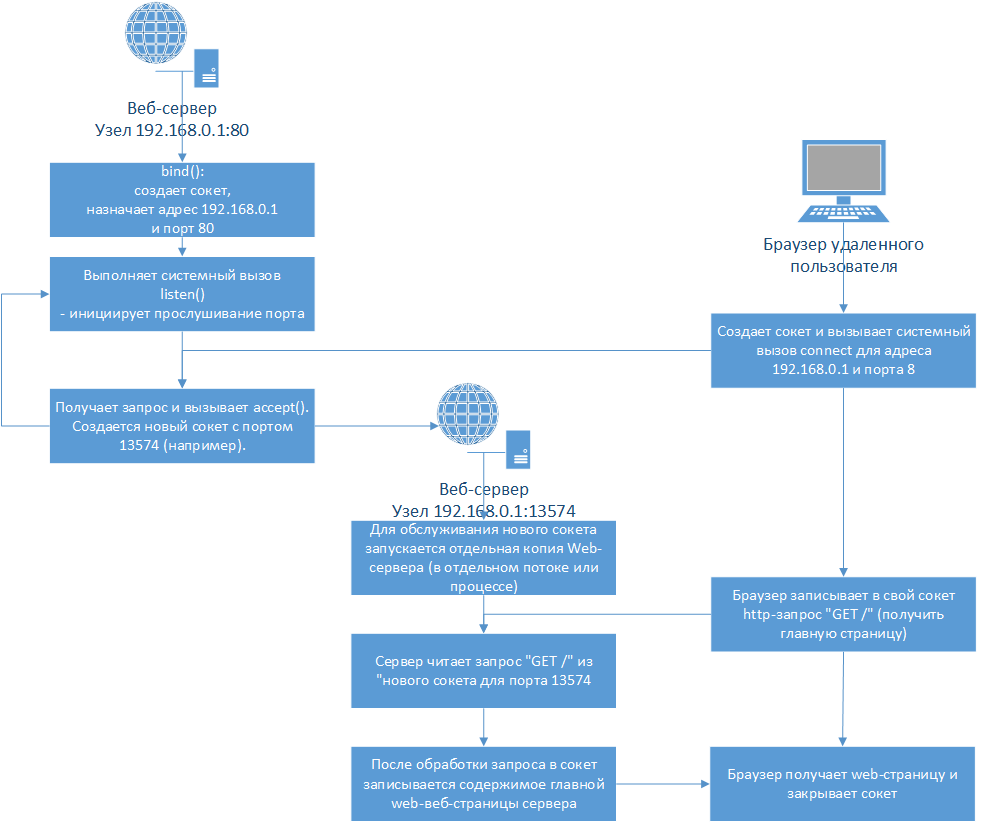
\includegraphics[scale=0.4]{images/lec12-pic05.png}
	\end{figure}
\end{frame}

\subsection{Соединение сокетов}

\begin{frame}[fragile]{Соединение сокетов}
	При использовании потоковых сокетов между взаимодействующими процессами должно сначала установиться соединение.
	Для этого клиент вызывает системный вызов connect():
	\begin{alltt}
		int connect (int FD, const struct sockaddr * SADDR,
                     socklen_t LEN);
	\end{alltt}
	\begin{itemize}
		\item FD - это дескриптор сокета;
		\item SADDR - указатель на структуру, содержащую сведения об адресе сервера;
		\item LEN - размер адресной структуры.		
	\end{itemize}
	Пример getwwwpage.c
	\begin{alltt}
		\$ gcc -o getwwwpage getwwwpage.c
		\$ ./getwwwpage bhv.ru > index.html
	\end{alltt}	
\end{frame}

\subsection{Прослушивание сокета}

\begin{frame}[fragile]{Прослушивание сокета}
	При взаимодействии через потоковые сокеты сервер должен включить прослушивание, т. е. перейти в режим ожидания запросов на подключение при помощи системного вызова listen():
	\begin{alltt}
		int listen (int FD, int QUEUE_LEN);
	\end{alltt}
	\begin{itemize}
		\item FD - это дескриптор сокета;
		\item QUEUE\_LEN определяет максимальный размер очереди запросов на подключение.
	\end{itemize}
	\begin{alltt}
		if (listen (sock, QUEUE_LENGTH) == -1) \{
		    fprintf (stderr, "listen() error");
		    return 0;
		\}
	\end{alltt}
\end{frame}

\begin{frame}[fragile]{Принятие запроса на подключение}
	\begin{itemize}
		\item Системный вызов listen() блокирует сервер до тех пор, пока какой-нибудь клиент не выдаст запрос на подключение. 
		\item Как только запрос поступил, сервер <<просыпается>>. 
		\item Если есть возможность обслужить запрос, то сервер вызывает системный вызов accept():
	\end{itemize}	
	\begin{alltt}
		int accept (int FD, struct sockaddr * ADDRESS, 
		            socklen_t * LENP);
	\end{alltt}
	\begin{itemize}
		\item FD - это дескриптор сокета;
		\item По адресу ADDRESS расположена структура, в которую помещаются адресные данные созданного соединения; 
		\item LENP — адрес переменной, в которую помещается размер адресной структуры.
	\end{itemize}

\end{frame}

\begin{frame}[fragile]
	Пример: socket2-server.c, socket2-client.c

	Вскоре после запуска сервер переходит в режим прослушивания сокета:
	\begin{alltt}
	\$ gcc -o socket2-server socket2-server.c
	\$ ./socket2-server
	\end{alltt}
	Откроем теперь другое терминальное окно и начнем передавать серверу запросы:
	\begin{alltt}
	\$ gcc -o socket2-client socket2-client.c
	\$ ./socket2-client Hello
	\$ ./socket2-client World
	\$ ./socket2-client Linux
	\end{alltt}	
	В исходном терминальном окне сервера будут выводиться соответствующие сообщения:
	\begin{alltt}
	>> Hello
	>> World
	>> Linux
	\end{alltt}	
	Сервер будет выводить сообщения, пока клиент не пошлет <<exit>>.
\end{frame}

\subsection{Прием и передача данных через сокеты}
\begin{frame}[fragile]{Прием и передача данных через сокеты}
	\begin{itemize}
		\item \textbf{Дейтаграммные сокеты} не предназначены для установки соединений посредством системных вызовов connect(), listen() и accept(). 
		\item Для передачи информации без использования соединений нужны системные вызовы, которые посылают и принимают данные через непосредственные адреса.
	\end{itemize}
	Для передачи данных на сервер через дейтаграммный сокет предусмотрен системный вызов sendto():
	\begin{alltt}
	ssize_t sendto (int FD, const void * BUFFER,
                    size_t BUF_SIZE, int FLAGS,
                    const struct sockaddr * SADDR,
                    socklen_t * LEN);
	\end{alltt}
	\begin{itemize}
		\item возвращаемое значение и первые три аргумента полностью идентичны тем, что используются в системном вызове write();
		\item FLAGS позволяет передавать дополнительные флаги; если таковых не имеется, пишите 0. 
		\item Через SADDR передается адресная структура сервера, на который посылаются данные. 
		\item LEN - это размер этой адресной структуры.
	\end{itemize}
\end{frame}

\subsection{Прием и передача данных через сокеты}
\begin{frame}[fragile]
	На серверной стороне данные принимаются при помощи системного вызова recvfrom():
	\begin{alltt}
        ssize_t recvfrom (int FD, void * BUFFER,
                          size_t BUF_SIZE, int FLAGS,
                          struct sockaddr * CADDR,
                          socklen_t * LENP)
	\end{alltt}
	\begin{itemize}
		\item системный вызов, кроме прочего, позволяет получить адрес отправителя, что важно в тех случаях, когда клиент ожидает ответ от сервера;
		\item возвращаемое значение и первые три аргумента полностью идентичны тем, что используются в системном вызове read();
		\item FLAGS позволяет передавать дополнительные флаги. 
		\item Через CADDR сервер может получить адресную структуру клиента. 
		\item LENP - это размер этой адресной структуры.
	\end{itemize}
	Пример: socket3-server.c, socket3-client.c
\end{frame}

\end{document} 
